\section{Monte Carlo-simulering}
\label{sec:mc}

\subsection{Varför simulera?}

En DCF ger ett tal, men talet är en funktion av antaganden som ingen känner. En
känslighetstabell varierar två av dem i taget. En Monte Carlo-simulering varierar alla på en
gång: man drar antagandena ur sannolikhetsfördelningar, räknar DCF:en en gång per dragning och
får en fördelning av värden i stället för ett tal. Här har du som matematiker ett försprång.
Det mesta är sannolikhetslära du redan kan, och det svåra är att vara ärlig med vad resultatet
betyder.

Motorn simulerar fyra drivare som \emph{förskjutningar} från basfallet: omsättningstillväxt och
EBITDA-marginal (samma förskjutning alla prognosår), WACC och evig tillväxt. Allt annat ligger
fast. Varje dragning värderas med samma funktion \kod{dcf_core} som basfallet, i ett enda
vektoriserat anrop utan slinga över simuleringarna.

\subsection{Val av fördelningar}

\begin{description}
  \item[Normalfördelning.] Naturlig för summan av många små störningar, men obegränsad. Det är
    ett problem här: en dragning med $\WACC \le g$ får Gordons formel att explodera.
  \item[Trunkerad normalfördelning.] En normalfördelning avskuren vid $\mu \pm 2\sigma$. Det är
    motorns standardval, eftersom den behåller klockformen men utesluter orimliga värden.
    Avskärningen sänker den faktiska standardavvikelsen till $0,88\sigma$.
  \item[Triangelfördelning.] Bestäms av minsta, troligaste och största värde. Den är lätt att
    fråga en expert om (”vad är det lägsta, troligaste och högsta du kan tänka dig?”) och får
    vara sned. En symmetrisk triangel med standardavvikelse $\sigma$ har halvbredden
    $\sqrt6\,\sigma$.
\end{description}

Alla tre dras med inversmetoden: om $U$ är likformig på $(0, 1)$ och $F$ är en
fördelningsfunktion har $X = F^{-1}(U)$ fördelningen $F$. För den trunkerade
normalfördelningen på $[a, b]$ är
$F^{-1}(u) = \mu + \sigma\,\Phi^{-1}\bigl(\Phi(\alpha) + u\,[\Phi(\beta) - \Phi(\alpha)]\bigr)$
med $\alpha = (a-\mu)/\sigma$ och $\beta = (b-\mu)/\sigma$.

\paragraph{Standardavvikelserna är antaganden.} Motorn sätter dem så här: tillväxt hälften av
den historiska standardavvikelsen i årlig tillväxt, marginal den historiska standardavvikelsen,
båda begränsade till 1 till 5 procentenheter, WACC 1 procentenhet och evig tillväxt 0,5. För
Atlas Copco är den historiska spridningen i tillväxt 14 procentenheter (tre observationer:
$+22$, $+2$ och $-5$\pct), så tillväxten slår i taket på 5. Marginalen har varierat så lite
(0,4 procentenheter) att den hamnar på golvet 1.

\subsection{Korrelerade dragningar: Cholesky och Gaussisk copula}

Drivarna är inte oberoende. Motorn antar att tillväxt och marginal samvarierar med
korrelationen $+0,3$ (ett bolag som växer fortare sprider sina fasta kostnader på fler sålda
enheter). Hur drar man korrelerade tal?

\paragraph{Steg 1: Cholesky.} Låt $z$ vara en vektor av oberoende standardnormala variabler, så
att $\E[z] = 0$ och $\Cov(z) = \E[z z\T] = I$. Låt $\Sigma$ vara den korrelationsmatris vi
vill ha. Eftersom $\Sigma$ är symmetrisk och positivt definit finns en entydig undre
triangulär matris $L$ med positiv diagonal så att $\Sigma = L L\T$
(Choleskyfaktoriseringen). Sätt $x = L z$. Då är
\begin{equation}
  \Cov(x) = \E\bigl[(Lz)(Lz)\T\bigr] = L\, \E[z z\T]\, L\T = L I L\T = \Sigma .
  \label{eq:cholesky}
\end{equation}
En linjär avbildning av en normalfördelad vektor är normalfördelad, så $x \sim N(0, \Sigma)$.
I två dimensioner med korrelation $\rho$:
\begin{equation}
  L = \begin{pmatrix} 1 & 0 \\ \rho & \sqrt{1-\rho^2} \end{pmatrix},
  \qquad x_1 = z_1, \quad x_2 = \rho z_1 + \sqrt{1-\rho^2}\, z_2 .
  \label{eq:cholesky2}
\end{equation}
Kravet på positiv definithet är inte en teknikalitet. En matris med parvisa korrelationer som
inte går ihop (A följer B, B följer C, men A går mot C) har ett negativt egenvärde, och då
finns ingen fördelning med de korrelationerna. Motorn kontrollerar det och ger ett begripligt
fel.

\paragraph{Steg 2: copula.} Cholesky ger korrelerade \emph{normalfördelade} tal, men drivarna
ska ha andra fördelningar. Lösningen är att gå via likformiga tal. Om $x_j \sim N(0, 1)$ är
$u_j = \Phi(x_j)$ likformig på $(0, 1)$, och $F_j^{-1}(u_j)$ har den önskade
marginalfördelningen $F_j$. Sambandet mellan variablerna följer med genom båda stegen, eftersom
båda avbildningarna är växande. Konstruktionen kallas Gaussisk copula: beroendet kommer från
en normalfördelning, marginalerna väljs fritt.

\begin{lstlisting}[caption={Dragningen i \texttt{run\_monte\_carlo} och copula-steget i
\texttt{\_transform}, \texttt{models/monte\_carlo.py}.},label=lst:mc]
rng = np.random.default_rng(config.seed)
cholesky = np.linalg.cholesky(correlation)
normals = rng.standard_normal((n, len(DRIVERS))) @ cholesky.T
offsets = {name: _transform(specs[name], normals[:, i]) for i, name in enumerate(DRIVERS)}

# in _transform: standard normal -> uniform -> marginal distribution
uniform = np.clip(ndtr(normals), _UNIFORM_EPS, 1.0 - _UNIFORM_EPS)
return _quantile(spec, uniform)
\end{lstlisting}

Raden \kod{@ cholesky.T} är~\eqref{eq:cholesky} för alla dragningar på en gång: varje rad i
matrisen är ett $z\T$, och $z\T L\T = (Lz)\T$. En detalj för den noggranne: korrelationen
anges på normalskalan. Rangkorrelationen bevaras exakt av de växande avbildningarna, men den
vanliga (Pearson) korrelationen mellan de färdiga drivarna blir något lägre än $0,3$ när
marginalerna inte är normala.

\subsection{Konvergens}

Medelvärdet av $n$ oberoende dragningar har enligt centrala gränsvärdessatsen medelfelet
\eng{standard error}
\begin{equation}
  \mathrm{SE}(\bar V_n) = \frac{s}{\sqrt{n}},
  \label{eq:se}
\end{equation}
där $s$ är stickprovets standardavvikelse. Felet avtar som $1/\sqrt{n}$: tio gånger bättre
precision kräver hundra gånger fler dragningar. Tabell~\ref{tab:konvergens} visar projektets
egna tal, och de följer regeln väl: mellan 687 och 10\,000 dragningar ökar $n$ med en faktor
14,6 och medelfelet faller med en faktor 3,8, mot väntade $\sqrt{14,6} = 3,8$.

\begin{table}[H]
\centering\small
\caption{Konvergens för Atlas Copco (slumpfrö 42, värde per aktie i kr, $s = 32,7$).}
\label{tab:konvergens}
\begin{tabular}{@{}rrrr@{}}
\toprule
Dragningar $n$ & Löpande medelvärde & Löpande median & Medelfel \\
\midrule
83 & 119,2 & 116,6 & 3,49 \\
687 & 121,6 & 116,6 & 1,24 \\
2\,812 & 121,3 & 116,2 & 0,62 \\
10\,000 & 121,6 & 116,7 & 0,33 \\
\bottomrule
\end{tabular}
\end{table}

Med 10\,000 dragningar är medelfelet 0,33\kr, eller 0,3\pct{} av värdet. Caset bekräftar det:
100\,000 dragningar med ett annat slumpfrö flyttar intervallet mellan 10:e och 90:e
percentilen från 84,3 till 164,9 till 84,0 till 165,2\kr. Simuleringen har alltså konvergerat.

\begin{komihag}
Precisionen i~\eqref{eq:se} gäller \emph{räknandet}, inte antagandena. Fler dragningar gör inte
standardavvikelserna mer rätt. I caset krymper intervallet från 84 till 165 till 90 till 155\kr{}
när tillväxtens standardavvikelse sänks från 5 till 3 procentenheter. Det är en
mångdubbelt större effekt än den av tio gånger fler dragningar.
\end{komihag}

\subsection{Varför medelvärdet ligger över basfallet: Jensens olikhet}

Simuleringen för Atlas Copco ger medianen 116,7\kr, nära basfallets 115,8, men medelvärdet
121,6. Det beror inte på att simuleringen har hittat en uppsida. För en konvex funktion $f$ och
en stokastisk variabel $X$ gäller Jensens olikhet:
\begin{equation}
  \E[f(X)] \ge f(\E[X]) .
  \label{eq:jensen}
\end{equation}
Gordon-värdet beter sig som $f(r) = 1/(r-g)$, som är konvex för $r > g$ eftersom
$f''(r) = 2/(r-g)^3 > 0$. Symmetrisk osäkerhet i $r$ ger därför en sned fördelning av värdet
med lång svans uppåt. Ett räkneexempel: med $g = 2$\pct{} och WACC antingen 6,65 eller
8,65\pct{} med lika sannolikhet blir $f$ antingen 21,5 eller 15,0. Medelvärdet 18,3 ligger
3,2\pct{} över $f(7,65\,\%) = 17,7$. Taylorutveckling till andra ordningen ger samma sak
allmänt: $\E[f(X)] \approx f(\mu) + \tfrac12 f''(\mu)\,\sigma^2$, det vill säga en relativ
höjning med $\sigma^2/(r-g)^2$. Därför redovisar motorn medianen, inte medelvärdet, som
centralt värde i football field.

\begin{figure}[ht]
\centering
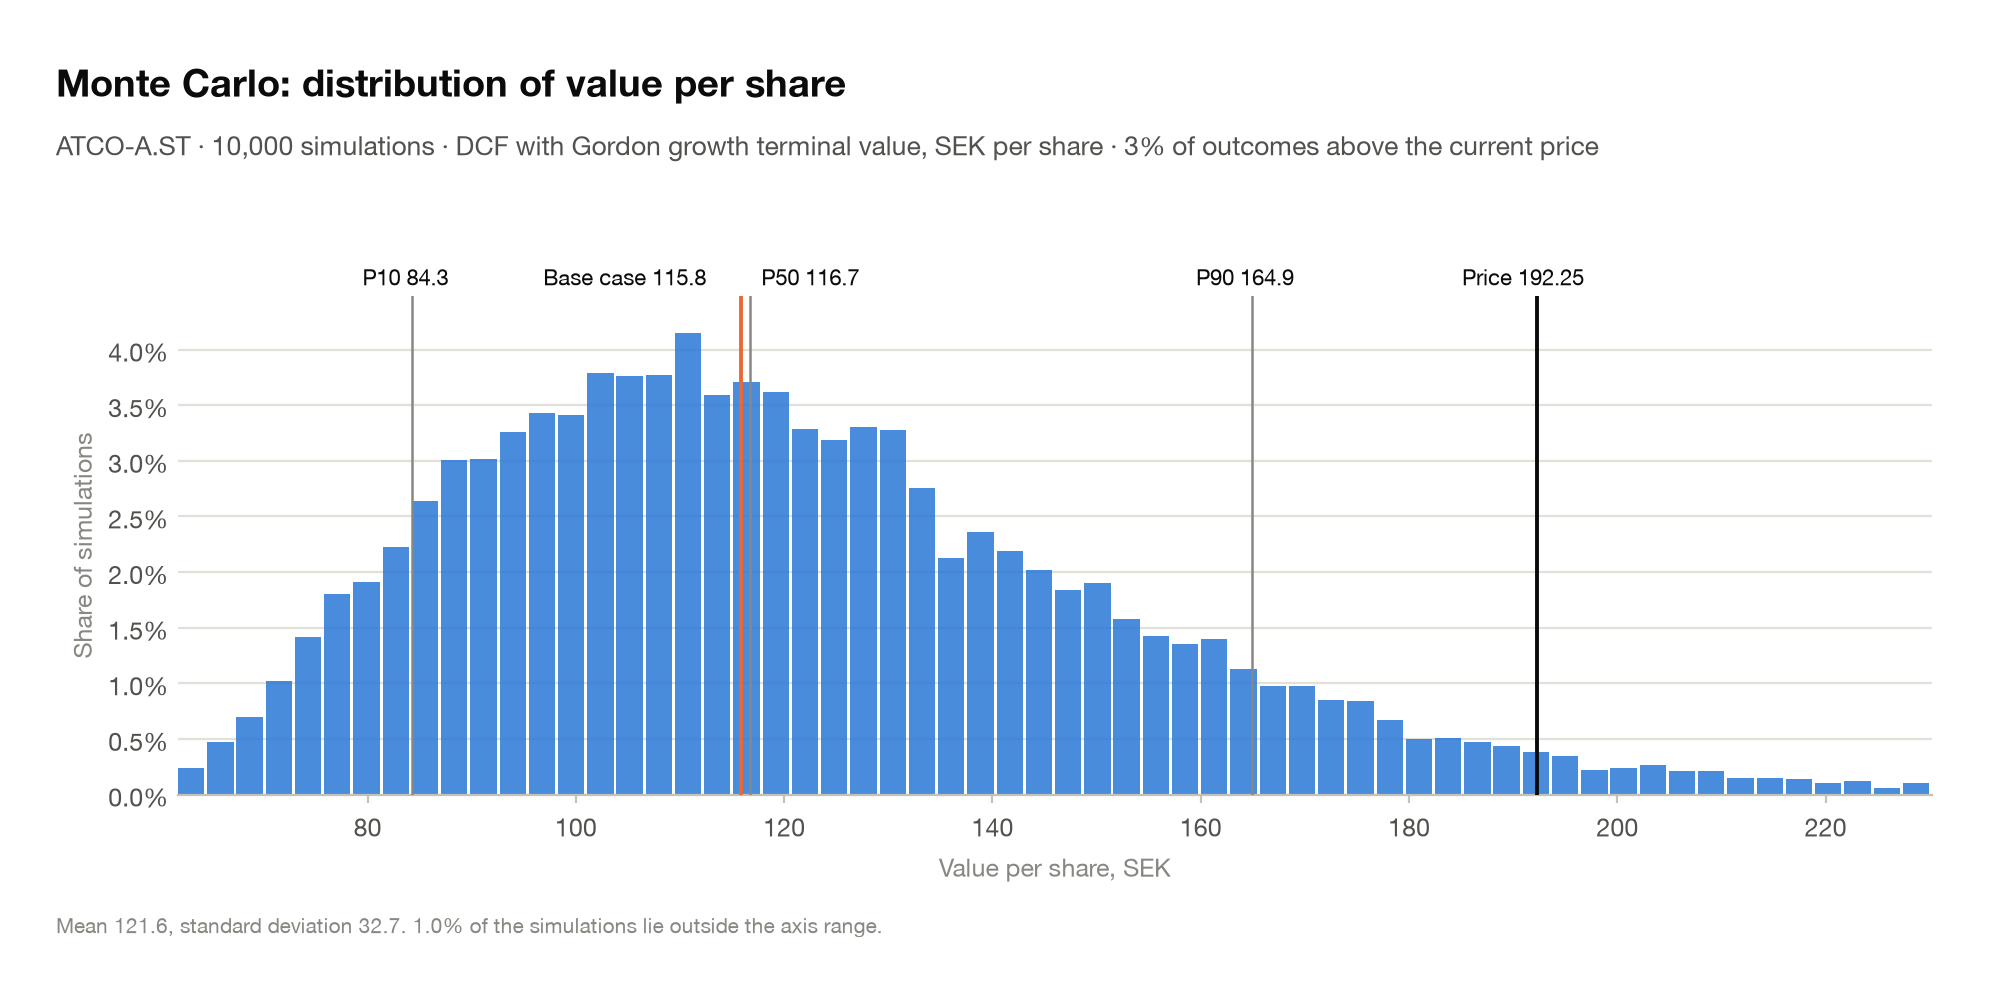
\includegraphics[width=0.95\linewidth]{mc_histogram.png}
\caption{Fördelningen av 10\,000 simulerade DCF-värden för Atlas Copco. Lägg märke till den
långa högersvansen.}
\label{fig:mc-hist}
\end{figure}

\subsection{Tornado och variansbidrag}

Två diagram visar vilka antaganden som betyder mest.

\paragraph{Tornadodiagrammet} (figur~\ref{fig:tornado}) ändrar en drivare i taget till sin 10:e
och 90:e percentil medan de andra ligger kvar i basfallet. För Atlas Copco flyttar tillväxten
värdet mellan 90,7 och 147,1\kr, WACC mellan 96,0 och 146,1, evig tillväxt mellan 107,6 och
126,0 och marginalen mellan 109,2 och 122,5.

\begin{figure}[ht]
\centering
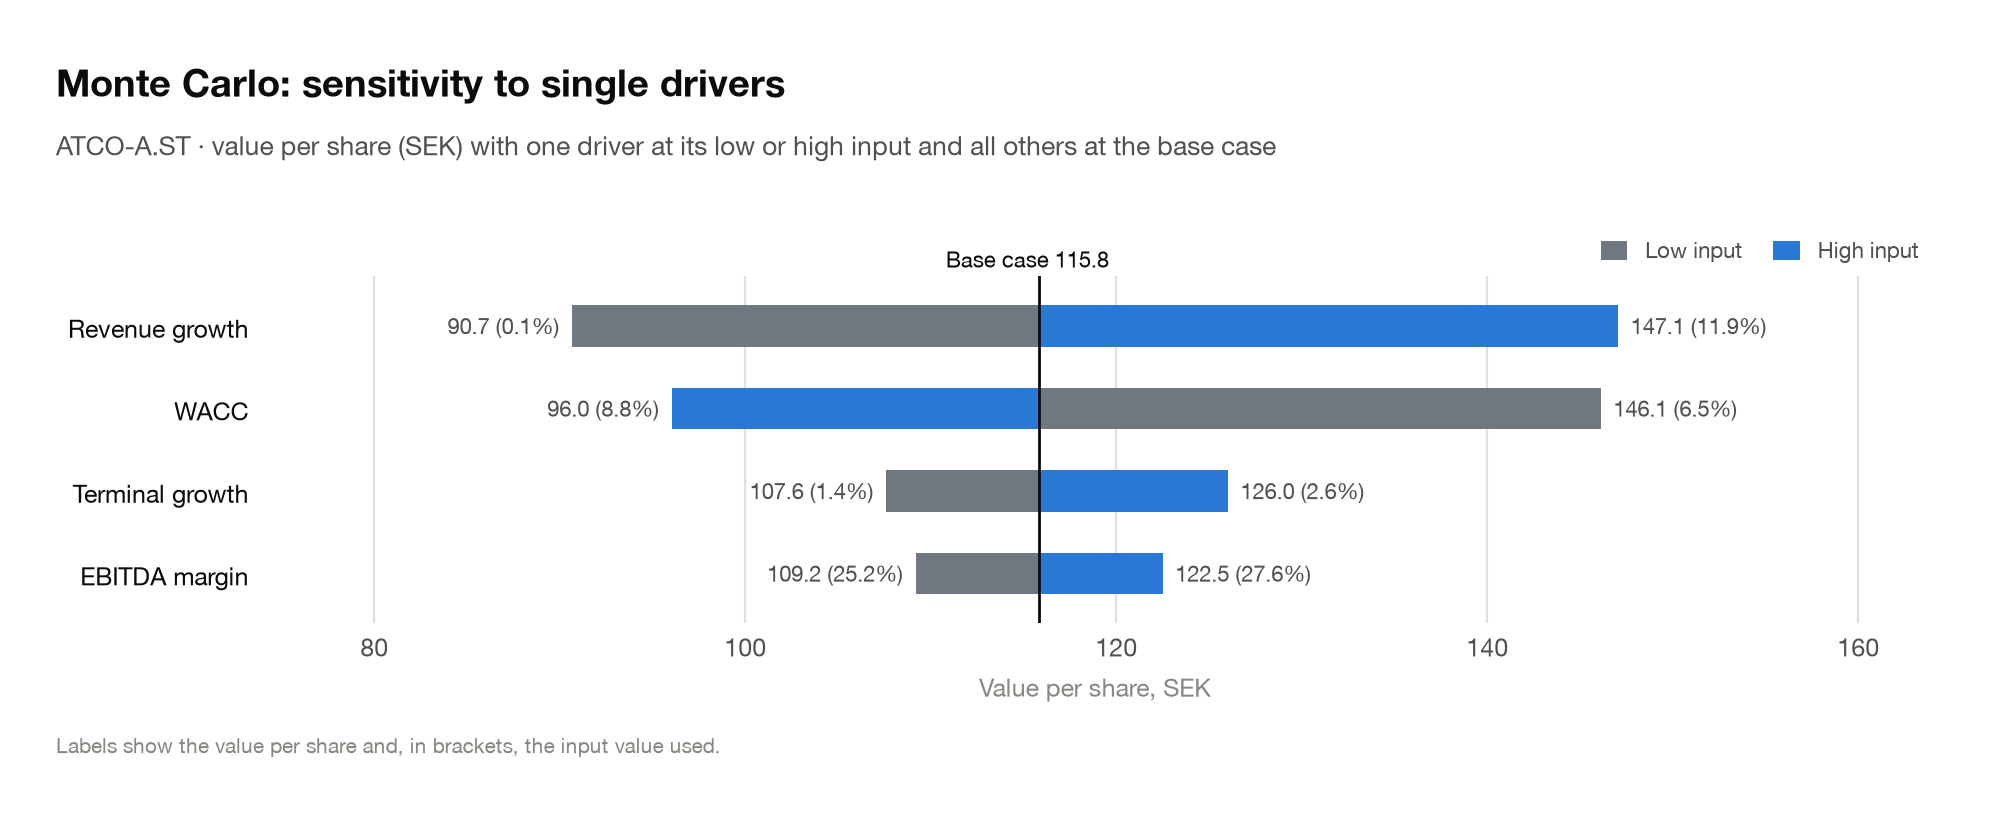
\includegraphics[width=0.95\linewidth]{mc_tornado.png}
\caption{Tornadodiagram: en drivare i taget mellan sin 10:e och 90:e percentil.}
\label{fig:tornado}
\end{figure}

\paragraph{Variansbidraget} mäts i motorn som den kvadrerade rangkorrelationen (Spearman)
mellan varje drivare och det simulerade värdet, normerad så att summan blir 1. För en linjär
modell med oberoende indata är den kvadrerade korrelationen precis drivarens andel av
variansen. Rangkorrelation används för att värdet är monotont men starkt olinjärt i WACC och
$g$. För Atlas Copco: tillväxt 51\pct, WACC 32\pct, marginal 12\pct{} och evig tillväxt 5\pct.

\begin{vanligtfel}
Att läsa in för mycket. (1) Båda diagrammen speglar de standardavvikelser man har matat in:
tillväxten väger tyngst delvis för att dess spridning ligger i taket. (2) Variansbidragen är
en rangordning, ingen riktig variansuppdelning. Med korrelerade indata överlappar de,
samspelseffekter (till exempel mellan WACC och $g$) syns inte, och normeringen döljer hur
mycket som inte förklaras alls. (3) Att 3,3\pct{} av dragningarna ligger över kursen är ingen
sannolikhet för att aktien är undervärderad. Det är ett påstående om modellen givet dess
antaganden.
\end{vanligtfel}
